% Conference submission version of main.tex.
% Two-column, ~8 pages. Written against a minimal TeX Live: no IEEEtran, no
% booktabs, no caption/xcolor, so the conference look is hand-rolled here and
% every optional package degrades gracefully.
%
%   pdflatex paper && pdflatex paper
%
% Figures come from make_figures.py so the plotted numbers and the numbers in
% the text have a single source.

\documentclass[10pt,twocolumn,letterpaper]{article}

\usepackage[margin=0.75in,columnsep=0.25in]{geometry}
% Times metrics are missing from this machine's TeX Live; uncomment on a full
% installation for the usual conference typeface.
\IfFileExists{ptmr7t.tfm}{\usepackage{times}}{}
\usepackage{amsmath}
\usepackage{amssymb}
\usepackage{amsthm}
\usepackage{graphicx}
\usepackage{array}
\usepackage{url}
\usepackage[hidelinks]{hyperref}

\IfFileExists{booktabs.sty}{\usepackage{booktabs}}{%
  \newcommand{\toprule}{\hline}
  \newcommand{\midrule}{\hline}
  \newcommand{\bottomrule}{\hline}
}
\IfFileExists{microtype.sty}{\usepackage{microtype}}{}

% --- conference-style captions (caption.sty is not available here) ---------
\makeatletter
\long\def\@makecaption#1#2{%
  \vskip\abovecaptionskip
  \small
  \sbox\@tempboxa{\textbf{#1.} #2}%
  \ifdim\wd\@tempboxa >\hsize
    \textbf{#1.} #2\par
  \else
    \global\@minipagefalse\hb@xt@\hsize{\hfil\box\@tempboxa\hfil}%
  \fi
  \vskip\belowcaptionskip}
\makeatother

% --- conference-style section headings ------------------------------------
\makeatletter
\renewcommand\section{\@startsection{section}{1}{\z@}%
  {-2.0ex \@plus -0.7ex \@minus -.2ex}{1.2ex \@plus.2ex}%
  {\centering\normalfont\large\bfseries}}
\renewcommand\subsection{\@startsection{subsection}{2}{\z@}%
  {-1.8ex\@plus -0.6ex \@minus -.2ex}{0.9ex \@plus .2ex}%
  {\normalfont\normalsize\bfseries}}
\makeatother
\renewcommand{\thesection}{\Roman{section}}
\renewcommand{\thesubsection}{\Alph{subsection}}
% headings print "A. Protocol"; cross-references read "Sec. V-A", as in IEEEtran
\makeatletter
\renewcommand{\p@subsection}{\thesection-}
\makeatother

\theoremstyle{plain}
\newtheorem{proposition}{Proposition}
\newtheorem{corollary}[proposition]{Corollary}

\newcommand{\xhat}{\hat{\mathbf{x}}}
\newcommand{\yhat}{\hat{\mathbf{y}}}
\newcommand{\zhat}{\hat{\mathbf{z}}}
\newcommand{\svec}{\mathbf{s}}
\newcommand{\gvec}{\mathbf{g}}
\newcommand{\SE}{\mathrm{SE}(3)}
\newcommand{\SOth}{\mathrm{SO}(3)}

\setlength{\abovecaptionskip}{6pt}
\setlength{\belowcaptionskip}{0pt}
\setlength{\textfloatsep}{12pt plus 2pt minus 2pt}

%The title deliberately does not promise a planner. A reviewer who forms that
%expectation in the abstract spends the rest of the paper arguing with it, and
%Table 1 shows RRT-Connect ahead by 54 points.
\title{\vspace{-1.2em}\bfseries\Large
Rigid-Body Symmetry in Flow-Matching Motion Planning:\\
What Canonicalisation Buys, and What It Does Not}

% Author order is a placeholder: student first, collaborator, supervisor last,
% which is the usual convention here but is not our call to fix. Confirm the
% order and that both co-authors have agreed to be listed before submitting.
\author{Andrea Sevincel \qquad Xinzhe Zhou \qquad Xiaoming Duan\\[2pt]
{\normalsize Shanghai Jiao Tong University}\\[1pt]
{\normalsize\texttt{aemirsevincel@gmail.com} \quad
\texttt{zhou\_xinzhe@sjtu.edu.cn} \quad \texttt{xduan@sjtu.edu.cn}}}

\date{}

\begin{document}
\maketitle

\begin{abstract}
\noindent
This is a controlled study of how to exploit rigid-body symmetry in a generative
motion planner, not a proposal for a competitive planner. Motion planning is
exactly equivariant under rigid transformations, and a substantial literature
builds that symmetry into network architectures. We hold the architecture, data
and training budget fixed, vary only the representation of the problem, and find
that almost all of the available benefit is obtained without touching the
architecture at all. We then measure how far the trained field departs from
equivariance, prove exactly what that quantity bounds --- the error any post-hoc
symmetrisation of a given model can remove --- and show what it does not bound:
two arms that are equally equivariant differ by $28$ points of held-out
performance. Equivariance of the learned field and performance are separable,
and the measurement sees only the first.

Our starting point is that the start and goal of a planning query themselves
define a frame, and that this frame removes five of the six degrees of freedom of
$\SE$ exactly, at zero computational cost. The sixth --- a roll about the
start--goal axis --- cannot be removed by any continuous rule; we give two
independent obstructions, one topological and one distributional. We therefore
treat the sixth by symmetry: roll augmentation during training and frame
averaging at inference.

The size of the effect is best read against a floor rather than in isolation. On
a cluttered 3D point-mass benchmark, world-frame flow matching reaches $15.4\%$
of individual samples collision-free on held-out environments --- statistically
indistinguishable from the $15.6\%$ obtained by joining start to goal with a
straight line, measured on the identical problems. Per sample, training on raw
world coordinates buys nothing over joining the endpoints with a line. With
the reduction, the same network, data and budget reach $45.6\%$, and,
contrary to the hypothesis that canonicalisation is a small-data crutch, the gap
\emph{widens} monotonically with training data: the world-frame arm gains $2.6$
points across a $12.5\times$ increase in training environments while the
canonicalised arm gains $26.6$ and has not plateaued.

The two mechanisms built for the sixth degree of freedom are worth almost
nothing: seed-matched across three runs, frame averaging contributes $+0.1$
points and roll augmentation $+0.8\pm0.3$, neither distinguishable from zero. A
translation-only reduction splits the $30.2$: recentring alone is worth $+12.3$
and aligning the axis a further $+18.0$. We explain this rather than merely reporting it,
by measuring the \emph{non-equivariance residual}: only $1.7\%$ of the learned
velocity field lies outside the equivariant subspace. Because frame averaging is
the orthogonal projection
onto that subspace, $1.7\%$ is the entire budget any post-hoc symmetrisation of
this model can spend. We propose the residual as a cheap diagnostic of how much
non-equivariant structure a learned field retains: it is one forward pass, needs
no retraining, and it quantifies the headroom available to post-hoc
symmetrisation exactly. The separation asserted above is measured, not assumed:
under the full $\SE$ action, augmentation and canonicalisation leave the field
equally equivariant ($r=0.018$ against $0.017$) while differing by $28$ points.

The obvious alternative --- exploiting the same symmetry by augmenting training
with random rigid motions --- recovers little of this: at $250$ environments it
lifts the world-frame arm from $15.4\%$ to $17.5\%$, about $7\%$ of what the
reduction achieves. We also find that optimisation and representation are
\emph{separate} bottlenecks: tripling the training budget is worth $+8.0$ points
to the canonicalised arm and $+0.9$ to the world-frame one, so compute cannot buy
what the representation forecloses --- and on the deployment metric the same
tripling moves the world-frame arm \emph{backwards}. The pattern replicates in a
second state space, an L-shaped rigid body whose state is a full pose rather than
a point: the world-frame arm fails to clear its own trivial floor in both
domains, the reduction clears it in both, and the ratio between arms is
$2.9\times$ in each. We calibrate both ends on the same $500$
problems: an untrained Brownian-bridge prior, swept over widths, never exceeds
$15.8\%$ at best-of-$20$, while classical planners reach $74$--$100\%$ in under
$0.4$\,s on one CPU core. The learned sampler
does not approach the latter, and we present this as a controlled study of
representation choices, not as a planner proposal.
\end{abstract}

\section{Introduction}

A motion planning problem consists of a workspace populated with obstacles, a
start configuration $\svec$, and a goal configuration $\gvec$; its solution is a
path $\tau$ joining them and avoiding the obstacles. The problem carries an exact
symmetry: for any rigid transformation $T \in \SE$,
\begin{equation}
  \tau\bigl(T\!\cdot\!\mathcal{O},\, T\svec,\, T\gvec\bigr)
  \;=\; T \cdot \tau\bigl(\mathcal{O},\, \svec,\, \gvec\bigr),
  \label{eq:equivariance}
\end{equation}
where $\mathcal{O}$ denotes the obstacle set. Nothing about the geometry changes
when the problem is picked up and moved.

A neural planner trained on raw world coordinates has no access to
Eq.~\eqref{eq:equivariance}. As far as its weights are concerned, planning
left-to-right near the ceiling is an unrelated task from planning front-to-back
near the floor, and the same skill must be relearned at every pose. The dominant
response in the literature is architectural: constrain the layers so that
equivariance holds by construction~\cite{cohen2016gcnn,thomas2018tfn,fuchs2020se3t,
deng2021vn,geiger2022e3nn}, an approach that has been carried into robot learning
with real success~\cite{ryu2023edf,wang2024equidp,simeonov2022ndf,yang2024equibot}.
That success comes at a price that is rarely quantified: constrained layers cost
expressiveness, are laborious to implement, and fail in ways that are silent.

There is a second route, older and much cheaper: build the symmetry into the
\emph{representation of the problem}, so that the network is never shown the pose
and therefore cannot be sensitive to it~\cite{puny2022fa,kaba2023canon}. This
paper asks how far that route goes on a generative motion planning problem, and
what can --- and cannot --- be inferred from measuring how equivariant a trained
model already is.

Our answer has four parts.

\textbf{(i) Five of six degrees of freedom are free.} The query supplies a frame.
Placing the origin at the midpoint of $\svec$ and $\gvec$ and aligning the first
axis with the start--goal direction removes three translational and two rotational
degrees of freedom, exactly and at no cost. The resulting representation is
invariant under any rigid transformation of the problem \emph{up to a single
roll about the start--goal axis}. The quantities a roll leaves alone --- the
separation $d$, the first coordinate of every reduced point, and its radius in
the plane normal to that axis --- are invariant outright
(Proposition~\ref{prop:exact}). Within those five that
is a stronger guarantee than a trained equivariant architecture provides, since
it holds to floating-point precision at initialisation rather than to
optimisation tolerance. The reduction therefore collapses $\SE$ to
$\mathrm{SO}(2)$; the remaining roll is what the rest of the paper is about. As
a side effect the six numbers previously used to condition the network on the
query collapse to a single invariant scalar.

\textbf{(ii) The sixth is provably not removable, for two unrelated reasons.} No
continuous rule can fix the roll about the start--goal axis: such a rule is a
nowhere-vanishing tangent field on $S^2$, which the hairy ball theorem forbids
(Proposition~\ref{prop:hairy}). Deriving the roll from the scene instead also
fails, because the obstacle distribution is symmetric under central inversion, so
the first angular moment --- the one a scene-derived gauge would actually use ---
vanishes in expectation for every start--goal direction
(Proposition~\ref{prop:moments}). We therefore handle the sixth degree of freedom
by symmetry rather than canonicalisation.

\textbf{(iii) The symmetry machinery buys little, and we measure why.} Roll
augmentation and frame averaging contribute $+0.8$ and $+0.1$ percentage points,
neither distinguishable from zero across three seed-matched runs, while the
reduction contributes $+30.2$. Rather than infer
inertness from flat curves --- a weak conclusion --- we measure the quantity frame
averaging exists to remove. The \emph{non-equivariance residual}, the disagreement
among rotated copies of the velocity field, is $1.7\%$ and is flat across a
$12.5\times$ range of training data. Since frame averaging is
the orthogonal projection onto the equivariant subspace
(Proposition~\ref{prop:fa}), the error it can remove is bounded by that $1.7\%$
(Corollary~\ref{cor:budget}), while the model is failing on most of its samples:
the model's error is overwhelmingly equivariant error.

\textbf{(iv) Calibration against floors and ceilings.} A collision-free rate is
uninterpretable on a new benchmark, so we measure, on the identical $500$ held-out
problems, both a trivial lower bound and four classical planners. The trivial
bound is the finding: a straight line from start to goal is collision-free on
$15.6\%$ of problems, and the world-frame model scores $15.4\%$ per sample. The
classical planners ($74$--$100\%$, all under $0.4$\,s on a single CPU core) bound
the other side and show that the learned sampler, at $45.6\%$, is not competitive
with them here. Because a generative planner is deployed as best-of-$N$ behind a
collision check, we also report that per-query metric against the honest control
for it --- the model's own untrained prior, sampled $N$ times, at its best width.
That comparison separates two things the per-sample number conflates: the
world-frame arm is at the straight-line floor per sample, but well above the
untrained prior per query, so it has learned sample \emph{diversity} without
learning sample \emph{quality}.

We regard (iii) as the transferable contribution. The residual is a few lines of
code, costs one forward pass, requires no retraining, and can be computed on any
model with a group action on its inputs. It converts ``we tried equivariance and
it did not help'' --- an anecdote --- into a quantitative statement about how much
headroom \emph{post-hoc symmetrisation} has on a given problem, with an exact
bound attached. We recommend it as a diagnostic to run before reaching for
symmetrisation, and we are explicit about its limit: measured across three arms
of this benchmark, $r$ does not predict what a symmetry mechanism is worth. Two
models with indistinguishable residuals differ by $28$ points
(Table~\ref{tab:twosigns}), because one of them fixed the representation and the
other only learned the symmetry.

\section{Related Work}

\textbf{Equivariant architectures.} Group-equivariant convolution~\cite{cohen2016gcnn}
generalises translation weight-sharing to larger groups; for $\SOth$ and $\SE$ the
standard constructions are tensor field networks~\cite{thomas2018tfn},
$\SE$-Transformers~\cite{fuchs2020se3t}, vector neurons~\cite{deng2021vn}, and the
\texttt{e3nn} framework~\cite{geiger2022e3nn}; \cite{bronstein2021gdl} surveys the
area. In robot learning these ideas underpin neural descriptor
fields~\cite{simeonov2022ndf}, equivariant descriptor fields~\cite{ryu2023edf},
equivariant diffusion policy~\cite{wang2024equidp}, and $\mathrm{SIM}(3)$-equivariant
policies~\cite{yang2024equibot}. This work does not dispute those results; it
provides a measurement that indicates when they are the right instrument.

\textbf{Canonicalisation and frame averaging.} Frame averaging~\cite{puny2022fa}
obtains equivariance by averaging an unconstrained network over a set of frames
derived from the input, and learned canonicalisation~\cite{kaba2023canon} predicts
a single frame with a small auxiliary network. Both leave the backbone
unconstrained. Our $(\svec,\gvec)$ reduction is a canonicalisation in this sense,
with the distinguishing feature that the frame is not learned or searched but read
directly off the query, so five degrees of freedom are removed in closed form; the
obstruction of Proposition~\ref{prop:hairy} is precisely the reason the sixth
cannot be handled the same way, and is why we fall back to frame averaging there.

\textbf{Generative motion planning.} Diffusion and flow models over whole
trajectories have become a standard planning
substrate~\cite{janner2022diffuser,chi2023dp,carvalho2023mpd,urain2023se3dif}. We
use the conditional flow matching / rectified flow
formulation~\cite{lipman2023fm,liu2023rectified,albergo2023interpolants} for its
straight-line interpolants and few-step sampling. Learned planners that regress
directly to paths~\cite{qureshi2019mpnet,fishman2022mpinets} form the
non-generative counterpart. Within this planning literature we are not aware of a
reported measurement of how far the learned field departs from equivariance.

\textbf{Measuring learned equivariance.} The idea of measuring, rather than
assuming, how equivariant a trained network is, is not new, and the closest
work to ours is outside planning. Gruver et al.~\cite{gruver2023lie} measure
learned equivariance through the Lie derivative of a trained model with respect
to the group action, and find that unconstrained architectures often acquire
substantial equivariance from data alone --- the same qualitative phenomenon our
residual reports, in a different parameterisation and for continuous groups.
Elesedy and Zaidi~\cite{elesedy2021strict} analyse the generalisation benefit of
equivariance using the orthogonal decomposition of a function into equivariant
and anti-equivariant parts, which is the decomposition
Corollary~\ref{cor:budget} is stated in. Relative to these, what we add is
narrow and practical: the residual is a single forward pass with no
differentiation and no retraining, and it comes with an exact statement of what
it bounds. We are careful not to claim more: it measures the headroom for
symmetrising a \emph{given} model, which is not the same question as how much a
constrained architecture would gain.

\textbf{Classical planners} supply our supervision: RRT-Connect~\cite{kuffner2000rrtconnect}
for feasibility, then shortcutting and CHOMP~\cite{zucker2013chomp} refinement, with
TrajOpt~\cite{schulman2014trajopt} available in the benchmark.

\section{Problem Setup}

\subsection{Benchmark}

Experiments use PointMass3D, a benchmark we built for this study. A spherical
robot of radius $0.03$ moves in the workspace $[-1,1]^3$ populated with $20$
spheres and $20$ axis-aligned boxes per environment, obstacle centres drawn
uniformly in $[-0.75,0.75]^3$. Collision checking uses an analytic signed distance
field: the environment SDF is the minimum over obstacle SDFs and the workspace
walls, and clearance subtracts the robot radius. Start and goal are drawn
uniformly subject to a collision margin and a minimum separation
$\|\gvec-\svec\| \ge 1.5$. Forty obstacles in a two-unit cube is dense clutter;
absolute success rates are correspondingly low and should be read comparatively.

Expert demonstrations come from RRT-Connect, random shortcutting, uniform
resampling to $64$ waypoints, and CHOMP refinement, with dense collision
validation and fallback to the raw RRT path. The dataset is $300$ environments
$\times\ 600$ start--goal pairs $\times\ 30$ trajectories, doubled by
time-reversal.

\subsection{Flow-matching planner}

The planner is a conditional flow-matching model over whole trajectories. A
trajectory is $N=64$ waypoints in $\mathbb{R}^3$. Training draws
$\mathbf{x}_0\sim\mathcal{N}(0,I)$ and $t\sim\mathcal{U}[0,1]$, forms the
interpolant $\mathbf{x}_t=(1-t)\mathbf{x}_0+t\,\mathbf{x}_1$ with $\mathbf{x}_1$
an expert trajectory, and regresses the velocity target:
\begin{equation}
  \mathcal{L}=\mathbb{E}_{\mathbf{x}_0,\mathbf{x}_1,t}
  \bigl\|v_\theta(\mathbf{x}_t,t,c)-(\mathbf{x}_1-\mathbf{x}_0)\bigr\|^2 ,
  \label{eq:cfm}
\end{equation}
where $c$ encodes the obstacles and the query. Sampling integrates
$\dot{\mathbf{x}}=v_\theta(\mathbf{x},t,c)$ from $t=0$ to $1$ by explicit Euler.
The network is a dilated temporal convolutional trunk with FiLM
conditioning~\cite{oord2016wavenet,perez2018film} fed by a PointNet-style
permutation-invariant obstacle encoder~\cite{qi2017pointnet}; $2.16$M parameters
throughout.

\section{Method}

\subsection{Decomposing the group}

$\SE$ has six degrees of freedom. The query supplies a frame, and that frame
consumes five of them:
\begin{itemize}\itemsep2pt
  \item \textbf{Three translations}, removed by placing the origin at the midpoint
        $\mathbf{o}=\tfrac12(\svec+\gvec)$.
  \item \textbf{Two rotations}, removed by aligning the first axis with
        $\xhat=(\gvec-\svec)/\|\gvec-\svec\|$. Specifying a direction on $S^2$
        costs exactly two degrees of freedom.
  \item \textbf{One rotation remains}: the roll about $\xhat$. Having fixed which
        way the path runs, nothing in the problem specifies which way is ``up''
        around that axis.
\end{itemize}

Concretely, let $d=\|\gvec-\svec\|$, let $i^\ast=\arg\min_i|\xhat_i|$, and set
\begin{equation}
  \yhat \propto \xhat\times\mathbf{e}_{i^\ast},
  \qquad
  \zhat = \xhat\times\yhat ,
  \label{eq:frame}
\end{equation}
with $R$ the rotation whose rows are $\xhat,\yhat,\zhat$. A point $\mathbf{p}$ maps
to $R(\mathbf{p}-\mathbf{o})$. Because the smallest component of a unit vector
satisfies $|\xhat_{i^\ast}|\le 1/\sqrt3$, the cross product in
Eq.~\eqref{eq:frame} has norm $\ge\sqrt{2/3}\approx0.816$ everywhere, so the
construction is well-conditioned over the entire domain with no threshold or
fallback branch, and $\det R=+1$ by construction.

\begin{proposition}[$\SE$ reduces to a single roll]
\label{prop:exact}
Let $X$ denote the reduced representation of $(\mathcal{O},\svec,\gvec)$ and $X'$
that of $(T\mathcal{O},T\svec,T\gvec)$ for $T=(Q,\mathbf{t})\in\SE$. Then there is
a single angle $\theta(T,\svec,\gvec)$ such that
\begin{equation}
  X' \;=\; R_{\xhat}(\theta)\, X ,
  \label{eq:prop1}
\end{equation}
where $R_{\xhat}(\theta)$ is the rotation by $\theta$ about the first axis,
applied to every reduced quantity --- waypoints, obstacle centres and obstacle
edge vectors alike. Consequently $d$, the first coordinate of every reduced
point, and its radius in the plane normal to that axis are invariant under all of
$\SE$; the residual ambiguity is exactly one degree of freedom.
\end{proposition}

\begin{proof}[Proof sketch]
Under $T$ the midpoint maps to $Q\mathbf{o}+\mathbf{t}$ and the direction to
$Q\xhat$, so both frames send the start--goal direction to the first basis
vector. A change of basis between two right-handed orthonormal frames that agree
on their first axis is a rotation about that axis, which gives
Eq.~\eqref{eq:prop1}; the invariants named are exactly the invariants of that
rotation.
\end{proof}

It is worth being precise about what this does \emph{not} say, because the
stronger claim is tempting and false. The reduced representation is not invariant
under $\SE$. The gauge $\yhat$ in Eq.~\eqref{eq:frame} is built from a
\emph{fixed world axis} $\mathbf{e}_{i^\ast}$, so rotating the whole problem
changes which axis is selected and rolls the frame. What Proposition~\ref{prop:exact}
establishes is that the entire residual is that one roll --- $\SE$ collapses to
$\mathrm{SO}(2)$, not to nothing. Five degrees of freedom are removed exactly, to
floating-point precision, at initialisation and without any training; the sixth
survives as a gauge ambiguity. This is precisely why the mechanisms of
Sec.~\ref{sec:sixth} exist, and a reader who took the representation to be fully
invariant would find those mechanisms unmotivated. We verify
Eq.~\eqref{eq:prop1} numerically to $10^{-15}$ in both domains.

Two further consequences follow. The six numbers $(\svec,\gvec)$ collapse to the
single invariant scalar $d$, and every pair of training examples that were ``the
same problem in a different pose'' now coincide up to a roll, raising the
effective density of the training set without generating a single new trajectory.

\subsection{Why the sixth degree of freedom is not removable}
\label{sec:moments}

\begin{proposition}[Topological obstruction]
\label{prop:hairy}
There is no continuous map $\yhat:S^2\to S^2$ with $\yhat(\xhat)\perp\xhat$ for
all $\xhat$. More generally, for a gauge $\yhat(\xhat,\mathcal{O})$ that may also
depend on the scene, fix any $\mathcal{O}$: then $\xhat\mapsto\yhat(\xhat,\mathcal{O})$
is a tangent field on $S^2$, and if continuous it vanishes somewhere.
\end{proposition}

\begin{proof}
Such a map is a continuous nowhere-vanishing unit tangent vector field on $S^2$,
whose existence the hairy ball theorem denies~\cite{milnor1978hairy}. The second
statement is the first applied to the section at fixed $\mathcal{O}$.
\end{proof}

The second form is what the scene-derived gauges of Sec.~\ref{sec:moments} need,
and it is worth being precise about what it gives. Such a gauge is a function of
$(\xhat,\mathcal{O})$, so the bare hairy ball theorem --- a statement about maps
out of $S^2$ alone --- does not apply to it. Fixing the scene repairs that, at
the cost of a weaker conclusion: the degenerate set is \emph{per scene}. Every
scene admits start--goal directions at which its gauge breaks down, but which
directions those are moves as the scene moves, so no restriction of the query
distribution can avoid them uniformly.

Every deterministic gauge therefore carries a discontinuity; one may relocate it
but never remove it. The escape route of restricting to a contractible subdomain
is closed here: the minimum separation $1.5$ along an axis of extent $2.0$ still
admits axis-aligned start--goal directions, so the domain is the whole sphere. Our
$i^\ast$ tie-break is exactly such a relocated discontinuity, placed on a
measure-zero set.

\begin{proposition}[Distributional obstruction]
\label{prop:moments}
Let the obstacle-centre law be invariant under the central inversion
$\mathbf{p}\mapsto-\mathbf{p}$, let $\varphi_j$ be the angles of the centres in
the plane normal to $\xhat$, and let the weights $w_j$ depend only on radius.
Then the angular moments $c_m=\sum_j w_j e^{im\varphi_j}$ satisfy
\begin{equation}
  \mathbb{E}[c_m] = 0 \quad\text{for every odd } m
  \text{ and every } \xhat \in S^2 .
  \label{eq:moments}
\end{equation}
\end{proposition}

\begin{proof}
Inversion fixes every radius and hence every $w_j$, and maps
$\varphi_j\mapsto\varphi_j+\pi$, so $e^{im\varphi_j}\mapsto(-1)^m e^{im\varphi_j}$
and $\mathbb{E}[c_m]=-\mathbb{E}[c_m]$ for odd $m$.
\end{proof}

The hypothesis is deliberately weaker than our benchmark: uniform-on-a-cube is
one centrally symmetric law, and the proof covers Gaussian clutter, spherical
shells, and any symmetric mixture equally. Nothing here is a theorem about our
own generator.

The restriction to odd $m$ is not a weakness of the proof but a fact about the
geometry, and it is worth stating because the natural stronger claim is false.
One is tempted to argue that the cube is $C_4$-symmetric, so only multiples of
four survive. That holds when $\xhat$ is a four-fold axis of the cube, and fails
otherwise, because the plane normal to a general $\xhat$ is not a coordinate
plane and the cube's symmetry group does not act on it as $C_4$. Numerically, at
$2\times10^5$ scenes (noise floor $0.002$), $|\mathbb{E}[c_2]|$ is $0.001$ along
a coordinate axis but $0.033$ for a generic direction and $0.070$ along a face
diagonal, while $|\mathbb{E}[c_1]|$ is at the noise floor for all of them.
Eq.~\eqref{eq:moments} is what the geometry actually supports.

Eq.~\eqref{eq:moments} is an \emph{unconditional} statement, and the gauge is
used conditionally --- a point that matters, and that closes the route more
firmly than the proposition alone. A scene-derived gauge is computed in the
reduced frame, i.e.\ from the displacements $\mathbf{p}_j-\mathbf{o}$ with
$\mathbf{o}=\tfrac12(\svec+\gvec)$. Conditional on the query, the law of
$\mathbf{p}_j-\mathbf{o}$ is the obstacle law shifted by $-\mathbf{o}$, which is
centrally symmetric about $-\mathbf{o}$ rather than about the origin. So
\begin{equation}
  \mathbb{E}[c_1 \mid \svec,\gvec] \;\neq\; 0
  \quad\text{whenever}\quad \mathbf{o}\neq\mathbf{0},
  \label{eq:cond}
\end{equation}
with the surviving moment pointing along the projection of $-\mathbf{o}$ onto
the plane normal to $\xhat$. Eq.~\eqref{eq:moments} recovers $\mathbb{E}[c_1]=0$
only after averaging over queries, since $\mathbb{E}[\mathbf{o}]=\mathbf{0}$. We
confirm Eq.~\eqref{eq:cond} numerically: at $\mathbf{o}=(0,0.4,0.3)$ the
conditional first moment has magnitude $0.56$ and argument $2.208$, against a
predicted $2.214$.

That is the sharper closing of the scene-derived route. Conditioned on a query
with $\mathbf{o}\neq\mathbf{0}$ the first-moment gauge is \emph{not}
degenerate --- it is well conditioned, and it points from the query midpoint
towards the centre of the workspace. But that direction is not an $\SE$-invariant
of the problem: it is a function of where the query sits in the world. A gauge
built on it would reintroduce exactly the world-frame dependence
Proposition~\ref{prop:exact} removes, forfeiting five degrees of freedom to fix
the sixth. The first-moment gauge is therefore either degenerate (unconditionally,
at $\mathbf{o}=\mathbf{0}$) or not equivariant (conditionally, elsewhere), and
neither is usable.

A gauge built from an even moment escapes Eq.~\eqref{eq:moments} --- inversion
does not kill even $m$ --- and also escapes Eq.~\eqref{eq:cond}, since an $m=2$
moment is insensitive to the sign of the displacement. It does not escape
Proposition~\ref{prop:hairy} in its second form: an $m=2$ moment defines a
\emph{director} rather than a vector, and a continuous director field on $S^2$ is
obstructed for the same Euler-characteristic reason as a vector field, since
$\chi(S^2)=2\neq0$. The conclusion is again per scene: for each fixed
$\mathcal{O}$ there are directions at which the director degenerates. Both routes
to a canonical roll are closed, for unrelated reasons.

\subsection{Handling the sixth by symmetry}
\label{sec:sixth}

\textbf{Roll augmentation.} During training a uniform $\theta\sim\mathcal{U}[0,2\pi)$
is composed into $R$, so reduction and roll are applied as a single rotation. The
prior $\mathbf{x}_0$ is drawn \emph{after} this rotation and never rotated: an
isotropic Gaussian is already rotation-invariant, so rotating it is a redundant
step capable only of introducing error.

\textbf{Frame averaging.} At inference the field is evaluated at $K$ rolled copies
of the state, each result rotated back, and averaged:
\begin{equation}
  (\mathcal{A}f)(\mathbf{x}) = \frac{1}{K}\sum_{k=0}^{K-1}
  \rho(\theta_k)^{-1} f\bigl(\rho(\theta_k)\mathbf{x}\bigr),
  \quad \theta_k=\frac{2\pi k}{K}.
  \label{eq:fa}
\end{equation}

\begin{proposition}[Exact $C_K$ equivariance and projection]
\label{prop:fa}
For any $f$, $\mathcal{A}f$ is exactly $C_K$-equivariant. Moreover $\mathcal{A}$
is linear, idempotent, and self-adjoint with respect to
$\langle f,g\rangle=\mathbb{E}_{\mathbf{x}}\left[f(\mathbf{x})^\top g(\mathbf{x})\right]$
for any $C_K$-invariant law on $\mathbf{x}$; hence it is the orthogonal projection
onto the subspace of $C_K$-equivariant fields.
\end{proposition}

\begin{proof}[Proof sketch]
Rolling the input by $\theta_j$ permutes the quadrature points, and reindexing a
finite sum is a bijection on them, giving equivariance and $\mathcal{A}^2=\mathcal{A}$.
Self-adjointness follows by substituting $\mathbf{x}\mapsto\rho(\theta_k)\mathbf{x}$
in the expectation, which the invariance of the law leaves unchanged, together
with $\rho(\theta_k)^\top=\rho(\theta_k)^{-1}$.
\end{proof}

We claim no novelty for Proposition~\ref{prop:fa} or for
Corollary~\ref{cor:budget} below. That group averaging is the orthogonal
projection onto the equivariant subspace, and that a function decomposes
orthogonally into equivariant and anti-equivariant parts, are established
results in the analysis of equivariant
learning~\cite{elesedy2021strict,puny2022fa}; we restate them because the
bound we are proposing is read off them. The contribution here is the
measurement --- the size of the anti-equivariant component of a trained planning
field, and what it implies for the mechanisms built to remove it --- rather than
the projection theorem.

Two properties of Eq.~\eqref{eq:fa} matter in practice. The guarantee requires no
architectural constraint and no training assumption --- it is a property of the
operator, and holds for an untrained network. And because the obstacle encoding is
time-independent, the $K$ rolled scene encodings are computed once outside the ODE
loop and reused at every integration step, which is why $K{=}9$ costs $1.05\times$
the wall-clock time of $K{=}1$ (Sec.~\ref{sec:cost}).

\subsection{The non-equivariance residual}
\label{sec:residual}

Proposition~\ref{prop:fa} turns a qualitative question --- ``is symmetry worth
enforcing here?'' --- into a measurable one. Write $v_k=\rho_k^{-1}f(\rho_k\mathbf{x})$
and $\bar v=\mathcal{A}f(\mathbf{x})$, and define
\begin{equation}
  r \;=\;
  \frac{\bigl(\mathbb{E}_{\mathbf{x},k}\bigl\|v_k-\bar v\bigr\|^2\bigr)^{1/2}}
       {\bigl(\mathbb{E}_{\mathbf{x}}\bigl\|\bar v\bigr\|^2\bigr)^{1/2}} .
  \label{eq:resid}
\end{equation}
This is the relative norm of the component of the learned field that lies outside
the equivariant subspace. The norms must be the Hilbert norms of
Proposition~\ref{prop:fa}, i.e.\ root-mean-square rather than mean-of-norms;
Jensen's inequality separates the two, and only the form in
Eq.~\eqref{eq:resid} makes Corollary~\ref{cor:budget} an identity rather than an
approximation.

\begin{corollary}[Symmetrisation budget]
\label{cor:budget}
Let $f^\ast$ be the target velocity field, which is $C_K$-equivariant because the
planning problem is. Since $\mathcal{A}$ is the orthogonal projection onto the
equivariant subspace and $\mathcal{A}f^\ast=f^\ast$, the error splits
orthogonally:
\begin{equation}
  \|f-f^\ast\|^2 \;=\; \underbrace{\|\mathcal{A}f-f^\ast\|^2}_{\text{equivariant error}}
  \;+\; \underbrace{\|(I-\mathcal{A})f\|^2}_{=\,r^2\|\mathcal{A}f\|^2}.
  \label{eq:budget}
\end{equation}
Hence \emph{(i)} the squared error that any equivariantisation of $f$ can remove
is at most $r^2\|\mathcal{A}f\|^2$, and $\mathcal{A}$ attains it; \emph{(ii)} the
remaining error $\|\mathcal{A}f-f^\ast\|$ is equivariant error, which no
symmetrisation of $f$ reduces; and \emph{(iii)} every map sending $f$ to an
equivariant field moves it by \emph{at least}
$\|f-\mathcal{A}f\|/\|f\| = r/\sqrt{1+r^2}$, with equality only for $\mathcal{A}$.
\end{corollary}

Part \emph{(iii)} is the direction the projection property actually gives, and it
is worth separating from \emph{(i)}: $\mathcal{A}f$ is the \emph{nearest}
equivariant field, so symmetrising is a lower bound on how much $f$ is disturbed,
never an upper one. What is bounded above is the \emph{error} that symmetrising
can remove, and only because the target is equivariant. Conflating the two --- as
an earlier version of this corollary did --- reverses the inequality.

The practical reading is narrower than a decision rule, and worth stating as
such. Measure $r$; if it is small, then by
Eq.~\eqref{eq:budget} the model's error is overwhelmingly \emph{equivariant}
error, and symmetrising $f$ --- by frame averaging, or by any other projection
onto the equivariant subspace --- can remove at most an $r^2$ fraction of the
field's squared magnitude from it. At the measured $r\approx0.017$ that is under
$3\times10^{-4}$, while
the model is failing on more than half of its samples: the two quantities are not
the same order, and no rearrangement of the symmetry can close the gap. The
measurement costs one forward pass and no retraining.

What it does not license is a verdict on building an equivariant architecture,
and on this point we can do better than a caveat. Symmetrising a trained field
and training a constrained model are different operations: the first is a
projection, bounded by Eq.~\eqref{eq:budget}; the second changes the hypothesis
class, and with it optimisation, capacity allocation and generalisation, none of
which $r$ measures.

We test that reading directly, and it fails: see
Sec.~\ref{sec:twosigns}, where two arms with indistinguishable residuals differ
by $28$ points of held-out performance.

This is also a consistency check on Proposition~\ref{prop:exact} for a
\emph{trained} model. For the reduced arm the $\SE$ residual is $0.0186$ at
$K{=}9$ and $0.0194$ at $K{=}32$, against $0.0191$ and $0.0192$ for the roll
residual at matched $K$: a rigid motion acts on the reduced representation only
through a roll, as claimed, and the two independently computed quantities agree
to $0.0005$. Table~\ref{tab:twosigns} quotes $K{=}8$, which is why its entry for
this arm ($0.0174$) differs slightly from the $K{=}9$ and $K{=}32$ values here;
the estimator is converged to within $0.002$ over that range.

We state the limit of this argument explicitly, because it is the objection a
reader should raise. Corollary~\ref{cor:budget} bounds what can be gained by
symmetrising \emph{this} model. It does not bound what an equivariant architecture
could achieve, since such an architecture searches a different hypothesis class
and may converge to a different --- possibly better --- equivariant field. What a
small $r$ does establish is that the model's residual error is overwhelmingly
\emph{within} the equivariant subspace, so \emph{projecting this model onto that
subspace} can remove very little of it. It does not follow that a constrained
architecture would gain little: Sec.~\ref{sec:twosigns} exhibits two arms that
satisfy the constraint equally well and differ by $28$ points, so membership of
that subspace is not what separates them.

\subsection{Implementation}
\label{sec:impl}

Three changes make the reduction representable, and one class of error had to be
designed out.

\textbf{Oriented boxes.} The reduction is a general $\SOth$ rotation, under which
an axis-aligned box becomes oriented. The usual six-number representation (centre,
half-extents) cannot express this. We use twelve numbers: a centre and three
half-edge \emph{vectors}, which in the world frame are $(h_x,0,0)$, $(0,h_y,0)$,
$(0,0,h_z)$, so the re-encoding is lossless. The environment SDF is unchanged,
since collision checking happens in the world frame after the inverse transform.

\textbf{Points and free vectors transform differently.} This is the error the
implementation is principally designed to prevent, because it fails silently.
Waypoints, endpoints, and obstacle centres are \emph{points} and take the affine
map $R(\mathbf{p}-\mathbf{o})$; the box half-edges are \emph{free vectors} and take
the rotation only, $R\mathbf{v}$. Applying the affine map to a half-edge adds
$-R\mathbf{o}$ to every edge --- identically --- so box \emph{position} survives
while box \emph{extent} is swamped by a common offset. The model goes blind to
obstacle size while the loss curve stays healthy. The severity scales with
$\|\mathbf{o}\|$, so the defect is invisible on exactly those problems whose
endpoints straddle the origin.

\textbf{Verification.} Eighteen tests cover deliberately disjoint failure classes.
Asserting $\svec,\gvec\mapsto(\mp d/2,0,0)$ catches translation errors, axis
ordering, and $R$ versus $R^\top$, but is blind to handedness, since a reflection
in the $y$--$z$ plane fixes the $x$-axis pointwise; $\det R>0$ covers that. Neither
detects the point/vector confusion, so a third test asserts
$\mathrm{featurise}(\rho\cdot S)=\mathrm{typed\_rotate}(\mathrm{featurise}(S),\rho)$
with the reference side written as explicit loops rather than the batched
operations under test, so it catches indexing and reshaping errors instead of
agreeing with them. A separate suite verifies Eq.~\eqref{eq:fa} against a
deliberately \emph{untrained} network --- the hard case, since
Proposition~\ref{prop:fa} should not depend on $f$.

One subtlety is worth recording for anyone measuring $r$. The group acts on the
whole input, scene and state together. An early version of our equivariance test
rolled only the state while leaving the conditioning in its original frame, and
reported a large violation from a correct implementation. A diagnostic written
that way manufactures the non-equivariance it claims to find.

\section{Experiments}

\subsection{Protocol}

All results use environments $250$--$299$, which no model was trained on,
evaluated as $50$ environments $\times\ 10$ start--goal pairs $\times\ 20$ samples
with $8$ Euler steps. The two arms are:

\begin{itemize}\itemsep2pt
  \item \textbf{Control}: world frame, conditioned on the raw pair $(\svec,\gvec)$.
  \item \textbf{Treatment}: the $(\svec,\gvec)$ reduction with uniform roll
        augmentation, conditioned on the invariant scalar $d$.
\end{itemize}

Both arms use the twelve-dimensional oriented-box representation, so it is not a
confound; both train on identical trajectories for $20$ epochs.

\textbf{Validation split.} Within training environments, validation holds out
whole start--goal pairs. A per-trajectory split leaks badly here: the $30$
trajectories per pair are near-duplicates (within-pair standard deviation $0.054$
against an overall $0.426$, because CHOMP is a local optimiser and converges to
the same route from similar initialisations). Under a per-trajectory split a
held-out trajectory has a training neighbour at RMS distance $0.030$; under the
pair split this rises to $0.162$.

\textbf{Two success metrics.} A sample is \emph{free} if the whole path is
collision-free. We report the per-sample rate throughout, because it is the
quantity the ablations compare and it is not inflated by drawing more samples.
The deployment metric is different: a generative planner is run as best-of-$N$
behind a collision check, so what a user experiences is the fraction of
\emph{queries} for which at least one of $N$ samples is free. We report that
separately in Sec.~\ref{sec:baselines}, where it can be compared against a
baseline that is also stochastic. Mixing the two is the main way this kind of
result gets overstated: at $N=20$ they differ by tens of points.

\textbf{Statistics.} We treat the number of \emph{distinct problems} ($500$) as
the sample size rather than the number of trajectories ($10{,}000$), since samples
within a problem and problems within an environment are correlated. This gives a
standard error of $\approx 2$ percentage points, and $\approx 2.7$ for a
difference of two arms. We checked that assumption rather than asserting it: a
bootstrap that resamples whole \emph{environments} --- the outermost correlated
unit --- gives a standard error of $2.2$ points on the $15.6\%$ straight-line rate
and $2.9$ on the $74.0\%$ TrajOpt rate (10{,}000 resamples), so the nominal figure
is if anything slightly conservative at the rates that matter here.

\textbf{Loss is not comparable across arms.} The treatment regresses targets in
the reduced frame, where trajectories are canonicalised along $+\xhat$, so its
target variance and hence its MSE are mechanically smaller. All reported
quantities are world-frame task metrics.

\subsection{Calibration: floors and ceilings}
\label{sec:baselines}

\begin{table}[t]
\centering
\footnotesize
\setlength{\tabcolsep}{3.5pt}
\begin{tabular}{lrrr}
\toprule
Planner & Free (\%) & Clearance & s/query \\
\midrule
straight line                   & 15.6 & 0.055 & $<0.001$ \\
TrajOpt                         & 74.0 & 0.026 & 0.352 \\
CHOMP                           & 88.8 & 0.019 & 0.394 \\
RRT-Connect                     & 99.6 & 0.017 & 0.284 \\
expert (RRT+CHOMP)              & 100.0 & 0.037 & 0.342 \\
\midrule
flow, world frame               & 15.4 & $-0.070$ & 0.067 \\
flow, $(\svec,\gvec)$ reduction & \textbf{45.6} & $-0.010$ & 0.067 \\
\bottomrule
\end{tabular}
\caption{The same $500$ held-out problems, solved five other ways. Classical
timings are one CPU core and one query; the learned rows are one GPU and $20$
samples per query, so the time column is not a like-for-like comparison.
Classical clearance is averaged over solved problems; the learned rows are
per-sample rates at $250$ training environments}
\label{tab:baselines}
\end{table}

\begin{figure}[t]
\centering
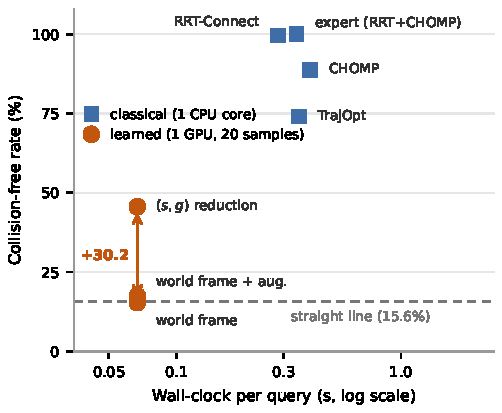
\includegraphics[width=\columnwidth]{fig_baselines.pdf}
\caption{Where the learned planner actually sits. The world-frame arm lies on the
straight-line floor; the reduction lifts it by $30.2$ points; the classical
planners remain far above. We show this rather than omit it: the contribution
here is the representation result, not a competitive planner}
\label{fig:baselines}
\end{figure}

A collision-free rate on a new benchmark means nothing without a scale, so we
built one. Table~\ref{tab:baselines} and Fig.~\ref{fig:baselines} report four
classical planners and a trivial baseline on the identical $500$ problems, using
the same collision checker. Classical planners are given one query at a time and
run single-threaded on one CPU core.

Two facts frame everything that follows.

\textbf{The floor.} A straight line from start to goal is collision-free on
$15.6\%$ of these problems --- the clutter is dense, but not so dense that the
direct path is usually blocked. The world-frame model reaches $15.4\%$ per sample.
The two are within $0.2$ points, an order of magnitude inside the standard error.
On a per-sample basis, whatever the world-frame arm has learned is worth nothing
over connecting the endpoints with a line. This is the sharpest available
statement of the problem the reduction solves, and it is invisible without the
trivial baseline.

\textbf{Augmentation is not the same lever.} The comparison above shows what
\emph{ignoring} the symmetry costs. The comparison a practitioner who already
knows about the symmetry would want is against the other standard way of using
it: augmenting the training distribution with random rigid motions of the whole
problem. We ran that arm at all four scales (Fig.~\ref{fig:scaling},
Table~\ref{tab:main}). It helps, it helps more as data grows --- augmentation
needs data to exploit --- and it is not close: $12.7$, $13.8$, $15.3$, $17.5$
against the reduction's $19.0$, $34.4$, $41.0$, $45.6$. At the largest scale
augmentation captures about $7\%$ of what canonicalisation does, and leaves the
world-frame arm within $2$ points of the straight-line floor. Making equivariance
\emph{likely} through the data is a different and much weaker mechanism than
removing the degrees of freedom outright.

\textbf{The stochastic floor.} A straight line has one sample, so it cannot be
compared against a best-of-$N$ number. The honest control there is the model's own
prior with the learning removed: Brownian bridges pinned at start and goal, drawn
$N=20$ times, filtered by the same collision check. We sweep the prior width and
report the \emph{best} setting, so the baseline is steel-manned
(Table~\ref{tab:prior}). Perturbing the straight line does not help. The best
best-of-$20$ result over the whole sweep is $15.8\%$ at $\sigma=0.05$, against
$15.6\%$ for the unperturbed line: random detours leave the workspace faster than
they route around anything, and by $\sigma=0.3$ the mean path is nine times longer
than the direct one and solves $2.2\%$. The $\sigma=0$ row also reproduces the
straight-line rate to the digit through an independent code path, which is a check
on both harnesses.

This changes the reading of the world-frame result in a way worth stating
carefully. Per sample, that arm is at the straight-line floor. Per query at $N=20$
it is not: the world-frame model trained on $20$ environments solves $44.8\%$ of
queries with at least one free sample, against $15.8\%$ for the best untrained
prior at the same $N$. So the world-frame model has learned something real --- its
samples are diverse in an informative way rather than a random one --- but it has
not learned to make any \emph{individual} sample better than a straight line. The
reduction is what closes that second gap.

\begin{table}[t]
\centering
\footnotesize
\setlength{\tabcolsep}{5pt}
\begin{tabular}{lrrrr}
\toprule
Prior width $\sigma$ & 0 & 0.05 & 0.10 & 0.30 \\
\midrule
per-sample free (\%)  & 15.6 & 11.5 & 7.4 & 0.4 \\
best-of-20 (\%)       & 15.6 & \textbf{15.8} & 13.4 & 2.2 \\
mean path length      & 1.79 & 3.31 & 5.86 & 16.85 \\
\bottomrule
\end{tabular}
\caption{The untrained stochastic baseline: Brownian bridges pinned at the
endpoints, $20$ samples per query, same collision check. Widening the prior buys
nothing at any setting, so best-of-$N$ over random detours is not what a learned
sampler is competing against}
\label{tab:prior}
\end{table}

\textbf{The ceiling.} RRT-Connect solves $99.6\%$ and the expert pipeline $100\%$,
in under $0.4$\,s of single-core CPU time; CHOMP from a straight-line
initialisation solves $88.8\%$. The learned sampler at $45.6\%$ is not competitive
with any of them. We report this plainly because the alternative --- comparing a
learned planner only against other learned planners --- is how a benchmark stops
measuring anything. The contribution of this paper is that the representation
change is worth $30$ points while the mechanisms built for the residual symmetry
are worth at most a few --- one indistinguishable from zero, the other unresolved.
That contribution does not require the planner to win, and we do not claim it
does.

\subsection{The reduction scales; the baseline does not}

\begin{table}[t]
\centering
\small
\setlength{\tabcolsep}{4.5pt}
\begin{tabular}{lrrrr}
\toprule
Training & \multicolumn{3}{c}{Collision-free (\%)} & best-of-20 \\
envs & World & {\footnotesize +aug.} & Reduction & Reduction \\
\midrule
20  & 12.8 & 12.7 & 19.0 & 57.8 \\
60  & 13.6 & 13.8 & 34.4 & 79.6 \\
150 & 14.6 & 15.3 & 41.0 & 85.6 \\
250 & 15.4 & 17.5 & \textbf{45.6} & \textbf{90.4} \\
\bottomrule
\end{tabular}
\caption{Held-out performance against training-set size. ``+aug.'' is the
world-frame arm trained with random $\SE$ motions of the whole problem. The
world-frame arm gains $2.6$ points across a $12.5\times$ increase in
environments and augmentation adds at most $2.1$ more, while the reduction gains
$26.6$ and has not plateaued. The $60$-environment row is a mean over three
seeds; the rest are single seed. The last column is the deployment metric,
best-of-$20$ behind a collision check}
\label{tab:main}
\end{table}

\begin{figure}[t]
\centering
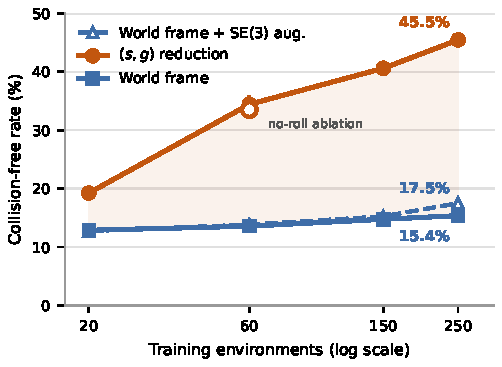
\includegraphics[width=\columnwidth]{fig_scaling_col.pdf}
\caption{The gap widens with data. If canonicalisation were compensating for a
shortage of training data one would expect it to close; instead the world-frame
baseline is nearly flat while the reduced model continues to improve. The hollow
marker is the no-roll ablation, drawn on the treatment line because it is the same
arm with one component removed}
\label{fig:scaling}
\end{figure}

Table~\ref{tab:main} and Fig.~\ref{fig:scaling} give the principal result. At
$250$ environments the reduction reaches $45.6\%$ against $15.4\%$, a gap of
$30.2$ points.

We state the uncertainty on that number conservatively, because the obvious
phrasing overstates it. Seeds were run at $60$ environments, not at $250$: the
seed-matched estimate there is $+20.9\pm1.6$ points ($n{=}3$ on both arms), which
is the only significance statement in this paper that rests on a measured seed
spread. The $30.2$ at $250$ environments rests on one seed per arm, and
expressing it as a multiple of a standard error measured in a different cell
would not be a valid test --- a $12.5\times$ change in training data is exactly
the kind of thing that can change run-to-run variance. We therefore report the
$250$-environment gap as a point estimate and rely on the $60$-environment cell,
where the comparison is seed-matched, for the inferential claim. Adding seeds at
$250$ environments is the cheapest open experiment in this project and we flag it
as such in Sec.~\ref{sec:limits}.

The trend is more informative than the endpoint. The baseline improves by $2.6$
points across a $12.5\times$ increase in training environments: it is close to
unable to exploit additional layouts, because each new layout arrives at poses it
must learn about separately. The reduction improves by $26.6$ points over the same
range and has not levelled off. This is the opposite of what a small-data-crutch
account predicts, under which the advantage should shrink as data accumulates.
Minimum clearance corroborates through an independent continuous measure: the
treatment moves from $-0.058$ toward $-0.0095$, approaching feasibility, while the
baseline is static.

Endpoint error falls by a factor of three to five under the reduction
($0.0101\!\to\!0.0041$ at $20$ environments, $0.0059\!\to\!0.0020$ at $250$), a
direct consequence of canonicalisation: with endpoints always at $(\mp d/2,0,0)$
the model no longer spends capacity on \emph{where} they are.

\subsection{Frame averaging is inert; the roll ablation is unresolved}

\begin{table}[t]
\centering
\footnotesize
\setlength{\tabcolsep}{4pt}
\begin{tabular}{lrl}
\toprule
Mechanism & $\Delta$ free & Assessment \\
\midrule
$(\svec,\gvec)$ reduction (5 DOF) & $+30.2$ pp & 1 seed at 250; $+20.9\pm1.6$ at 60 \\
\quad of which: 3 translations    & $+12.3$ pp & recentring alone \\
\quad of which: 2 rotations       & $+18.0$ pp & aligning the axis \\
$\SE$ augmentation (world frame)  & $+2.1$ pp  & real, but $7\%$ of the above \\
Roll augmentation                 & $+0.8$ pp  & $\pm0.3$ paired, $n{=}3$; n.s. \\
Frame averaging ($K{:}1\!\to\!3$) & $+0.1$ pp  & $0.05$ SE ($\approx 0$) \\
\bottomrule
\end{tabular}
\caption{Decomposition by mechanism on the same held-out set. Among the
mechanisms tested, canonicalisation accounts for the effect, and both parts of it
matter: recentring and axis alignment contribute $41\%$ and $59\%$ of the total.
Neither mechanism built for the sixth degree of freedom is distinguishable from
zero. The $\Delta$ column is against the arm without that mechanism, so the rows
are not additive; the two indented rows decompose the row above them}
\label{tab:ablation}
\end{table}

\begin{figure*}[t]
\centering
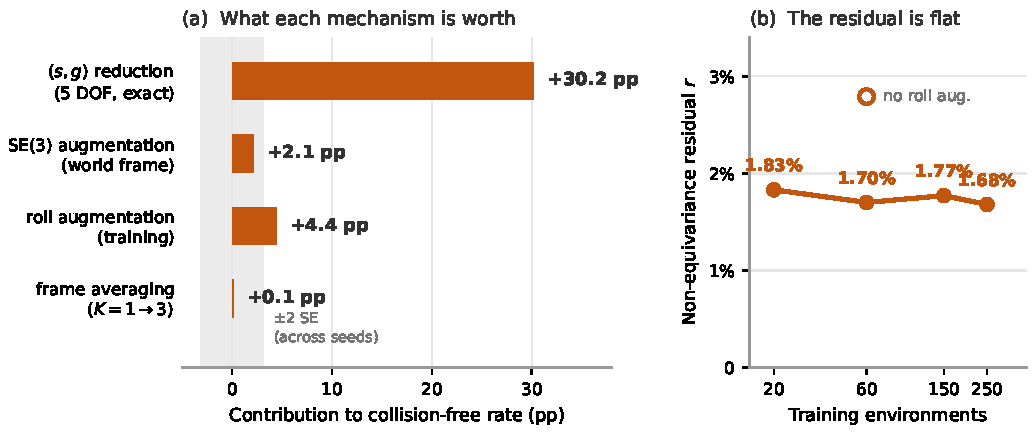
\includegraphics[width=0.92\textwidth]{fig_mechanisms.pdf}
\caption{(a) Canonicalisation is seven times the next largest mechanism. The band
is $\pm2$ across-seed standard errors, measured on the treatment arm at $60$
environments; frame averaging sits inside it, and the roll-augmentation bar rests
on a single-seed ablation. (b) The non-equivariance residual of
Eq.~\eqref{eq:resid} is flat across a $12.5\times$ range of training data --- it
is not something the model acquires from seeing more layouts. The hollow marker
shows that removing roll augmentation raises the residual by $64\%$ but leaves it
under $3\%$}
\label{fig:mechanisms}
\end{figure*}

Table~\ref{tab:ablation} and Fig.~\ref{fig:mechanisms}a decompose the result.
Removing roll augmentation (the reduction with a fixed gauge) costs $34.4\%$
against $33.5\%$ at $60$ environments. Both arms were run at the same three
seeds, so the comparison should be paired, and paired it is $+1.2$, $+0.2$ and
$+1.1$ points: a mean of $+0.8\pm0.3$, consistently positive but $t=2.6$ on two
degrees of freedom, which does not clear significance at $n{=}3$. Unpaired, the
across-arm spread swamps it entirely ($0.4$ SE). Frame averaging on the best
model gives $45.63\%$ at $K{=}1$ and $45.70\%$ at $K{=}3$ --- $0.05$ across-seed
standard errors.

The reduction itself decomposes. A translation-only variant, which recentres on
the query midpoint without rotating, reaches $27.7\%$ at $250$ environments,
between the world frame's $15.4\%$ and the full reduction's $45.6\%$. So the
three translational degrees of freedom are worth $+12.3$ points and the two
rotational ones a further $+18.0$: $41\%$ and $59\%$ of the total. Neither half
carries the effect on its own, which is worth knowing --- recentring is the
trivially easy part of the reduction, and it accounts for two fifths of the
benefit.

Rather than infer inertness from flat curves, we measure $r$. On the best model
$r=0.0168$ at $K{=}3$: under $2\%$ of the field is
non-equivariant. By Eq.~\eqref{eq:budget} the squared error any equivariantisation
can remove is at most $r^2$ of the field's squared magnitude, i.e.\ about
under $3\times10^{-4}$, while the model is failing on more than half of its
samples.
The remaining error respects the symmetry and is untouchable by symmetrisation.

Two observations sharpen this. First, removing roll augmentation raises the
residual by $64\%$ ($0.0170\!\to\!0.0279$ at $60$ environments) --- a large
relative change, but between two values that are both under $3\%$, so
augmentation is not what makes the field near-equivariant in the first place. The explanation is that the
gauge is a deterministic function of $\xhat$, and $600$ start--goal pairs per
environment supply $600$ distinct directions; the reduced-frame data already spans
a wide spread of rolls, and explicit augmentation was solving a problem the data
had already solved. Second, and contrary to what we expected, the residual does
\emph{not} move with scale: $0.0183$, $0.0170$, $0.0177$, $0.0168$ across a
$12.5\times$ range of training data (Fig.~\ref{fig:mechanisms}b). It is small and
flat. An earlier two-point reading under a mean-of-norms definition of $r$
suggested a downward trend; measured at four scales under Eq.~\eqref{eq:resid} it
is a constant, and we report it as one.

That the residual is flat rather than falling is itself informative. It means
the near-equivariance of the learned field is not something the model acquires
gradually from seeing more layouts --- it is present at $20$ environments and
unchanged at $250$. Combined with the no-roll ablation, the picture is that the
reduced-frame data supplies enough implicit roll diversity from the outset, and
that nothing about the scale of the training set changes how equivariant the
learned field is. What rests on the \emph{size} of $r$ and
Corollary~\ref{cor:budget} is the narrower conclusion that \emph{symmetrising
this model} cannot help, and that conclusion does not depend on a trend. It says
nothing about what a constrained architecture would achieve, for the reason
Sec.~\ref{sec:twosigns} makes concrete.

\subsection{What the residual does not predict}
\label{sec:twosigns}

To test the tempting reading directly we measured $r$ under the \emph{full}
$\SE$ action rather than the roll alone, which makes it defined for the
world-frame arm as well: $K$ random rigid motions are applied to the whole
problem, the field is evaluated in each, and each result is mapped back by the
inverse rotation. Table~\ref{tab:twosigns} is the result.

\begin{table}[t]
\centering
\small
\begin{tabular}{lrr}
\toprule
Arm (250 environments) & $r$ under $\SE$ & Free (\%) \\
\midrule
World frame                     & $0.0881$ & $15.4$ \\
World frame $+\ \SE$ augmentation & $0.0181$ & $17.5$ \\
$(\svec,\gvec)$ reduction         & $0.0174$ & $\mathbf{45.6}$ \\
\bottomrule
\end{tabular}
\caption{The residual does not predict what a mechanism is worth. Augmentation
and canonicalisation leave the learned field equally equivariant, and differ by
$28$ points of held-out performance}
\label{tab:twosigns}
\end{table}

Augmentation drives the residual down by a factor of $4.9$: it demonstrably
teaches the network the symmetry, to the same degree the reduction enforces it
by construction. It buys $2.1$ points. The reduction, at an indistinguishable
residual, buys $30.2$. \emph{Two models with the same $r$ can differ by $28$
points}, so $r$ does not forecast the benefit of a symmetry mechanism, and a
decision rule of the form ``build the constrained architecture only if $r$ is
large'' has no support here. What $r$ bounds is what symmetrising a given field
can remove, which is Eq.~\eqref{eq:budget} and is a theorem; what it does not
measure is whether symmetry is the binding constraint at all.

One number in Table~\ref{tab:twosigns} deserves saying out loud. The world-frame
arm ignores the symmetry entirely and performs at the straight-line floor --- and
it is still $91\%$ equivariant. A model that has learned nothing useful about
planning has nonetheless landed close to the equivariant subspace, because most
of what a velocity field does on this problem is roughly pose-independent
regardless of how it was trained. That is the sharpest form of the point: $r$
being small is compatible with having solved the problem, with having learned the
symmetry and nothing else, and with having learned nothing at all.

\subsection{How much of the level is training budget}
\label{sec:budget}

Every arm above is trained for $20$ epochs, and that budget is not enough. Holding
the data fixed at $60$ environments and training the reduced arm for $60$ epochs
instead raises the held-out collision-free rate from $34.4\%$ --- the mean over
three seeds --- to $\mathbf{42.4\%}$, with minimum clearance improving from
$-0.031$ to $-0.013$ and endpoint error from $0.0024$ to $0.0022$. Three times
the optimisation, at identical data and identical capacity, is worth $+8.0$
points, nearly twice the largest of the mechanisms built for the sixth degree of
freedom. Against the single seed the $20$-epoch cell was originally reported
from, the same comparison would read $+11.1$; we quote the seed mean throughout.

Two consequences follow, and the second is a correction.

First, this is the direct evidence that the absolute level is a budget artefact
rather than a ceiling of the method, and it is the evidence we rely on rather
than the train--validation comparison discussed in Sec.~\ref{sec:limits}. The
model at $20$ epochs is substantially underfit, so the $45.6\%$ headline
understates what this architecture reaches at convergence.

Second --- and this is the part we did not anticipate --- the same tripling is
worth almost nothing to the world-frame arm. Running it at $60$ epochs on the
same $60$ environments moves it from $13.6\%$ to $14.4\%$:
\begin{center}\small
\begin{tabular}{lrrr}
\toprule
$60$ environments & $20$ ep. & $60$ ep. & gain \\
\midrule
\multicolumn{4}{l}{\emph{per-sample collision-free (\%)}}\\
World frame            & $13.6$ & $14.4$ & $+0.9$ \\
$(\svec,\gvec)$ reduction & $34.4$ & $\mathbf{42.4}$ & $+8.0$ \\[2pt]
\multicolumn{4}{l}{\emph{best-of-20 (\%)}}\\
World frame            & $42.3$ & $39.2$ & $-3.1$ \\
$(\svec,\gvec)$ reduction & $79.6$ & $\mathbf{87.2}$ & $+7.6$ \\
\bottomrule
\end{tabular}
\end{center}
Optimisation buys $+8.0$ points with the reduction and $+0.9$ without it, an
interaction of $+7.1$ points at roughly $4.5$ across-seed standard errors. The
two mechanisms are not substitutes: they relieve different constraints. The
representation bottleneck --- the network being shown a pose it must relearn at
every value --- is removed by canonicalisation and \emph{cannot} be removed by
compute. The capacity bottleneck is removed by compute and cannot be removed by
canonicalisation. This also settles the reading of Fig.~\ref{fig:scaling}: the
world-frame arm's flatness is not an artefact of an insufficient budget, because
giving it three times the budget leaves it flat.

The deployment metric at this budget is high: best-of-$20$ behind a collision
check solves $\mathbf{87.2\%}$ of held-out queries, against $15.8\%$ for the best
untrained prior at the same $N$ (Table~\ref{tab:prior}). A reader who cares about
whether the sampler is useful rather than about the representation question
should read that number, with the caveat from Sec.~\ref{sec:baselines} that
classical planners still solve more of them and faster.

On that metric the interaction is not merely larger but changes sign for the
control. The reduction rises from $79.6\%$ to $87.2\%$, while the world-frame arm
\emph{falls}, from a three-seed mean of $42.3\%$ (spread $41.4$--$43.2$) to
$39.2\%$: an interaction of $+10.7$ points against the $+7.1$ measured per
sample. Tripling the optimisation of the world-frame arm made it worse on the
metric that describes how a generative planner is actually deployed --- more
training bought a per-sample gain of $+0.9$ while costing sample diversity, which
is the resource best-of-$N$ actually spends. We flag one caveat on our own
number: the $60$-epoch cells are single seed against three-seed means, which is
precisely the shape that manufactured the roll-augmentation artefact discussed in
Sec.~\ref{sec:limits}, so this $-3.1$ needs a seed-matched confirmation before it
is leaned on. The $+7.1$ per-sample interaction does not depend on it.

\textbf{This is a trend, not a limit.} Neither arm has been trained to a plateau,
so the strongest form of the objection --- that the gap reflects convergence
\emph{rate} rather than representation --- is answered here by two points rather
than by a limit. What the two points establish is the direction: the gap
\emph{widens} from $20.8$ to $28.0$ points under $3\times$ the budget, so if
undertraining were manufacturing the gap it is the flat arm that would have the
headroom, and it does not. A convergence study at $60$ environments is the
experiment that would close this, and we state in Sec.~\ref{sec:limits} what each
outcome would mean for the framing.

\subsection{Replication in a second state space}
\label{sec:se3}

\begin{table}[t]
\centering
\footnotesize
\setlength{\tabcolsep}{4pt}
\begin{tabular}{lrrrr}
\toprule
Domain (trivial floor) & World & Reduction & ratio & interaction \\
\midrule
$\SE$ rigid body ($4.8\%$) & $3.0$  & $8.6$  & $2.9\times$ & $+2.1$ \\
Point mass ($15.6\%$)      & $14.4$ & $42.4$ & $2.9\times$ & $+7.1$ \\
\bottomrule
\end{tabular}
\caption{The same pattern in a second state space. Per-sample collision-free
rates at $250$ environments and the longer training budget, each against the
trivial baseline for its own domain --- geodesic interpolation for the rigid
body, a straight line for the point mass. In both domains the world-frame arm
fails to clear its own floor and the reduction clears it; the ratio between arms
agrees to two figures; and the epoch-gain interaction of Sec.~\ref{sec:budget}
reproduces in sign and shape. Single seed per cell}
\label{tab:se3}
\end{table}

The point-mass domain has a convenient property that could be doing the work: the
state is a point, so the points-versus-vectors distinction of Sec.~\ref{sec:impl}
lives only in the obstacle features, never inside the trajectory. To test whether
the result survives without that convenience we built a second domain --- an
L-shaped rigid body in the same clutter, where a state is a full pose, position
and orientation, rather than a point. The trajectory now carries orientation, so
the typing distinction moves inside the state. Collision checking evaluates the
obstacle SDF at the body's transformed sphere centres; steering interpolates
linearly in position and geodesically in rotation; and the trivial baseline is
the corresponding geodesic interpolation, the $\SE$ analogue of joining start to
goal with a line.

Three things replicate (Table~\ref{tab:se3}). The world-frame arm fails to beat
the trivial baseline in \emph{both} domains --- $1.8$ points below the geodesic
floor here, $1.2$ below the straight-line floor there --- so the finding of
Sec.~\ref{sec:baselines} is not an accident of one workspace family. The
reduction clears its floor in both. And the ratio between the arms is $2.9\times$
in each, with the epoch-gain interaction reproducing in sign and shape.

We are deliberately careful about how much this carries. The absolute numbers are
small ($3.0\%$ and $8.6\%$ against a $4.8\%$ floor), a rigid body in this clutter
is a substantially harder problem than a point, and every $\SE$ cell is single
seed. The useful statement is the \emph{pattern}, not the level: the reduction is
not exploiting something peculiar to a point-shaped state, and the implementation
survives having the failure mode of Sec.~\ref{sec:impl} moved from the
conditioning into the trajectory itself, which is the part most likely to break
silently.

\subsection{Cost}
\label{sec:cost}

Frame averaging at $K{=}9$ costs $1.05\times$ the wall-clock time of $K{=}1$
($0.070$ vs $0.067$\,s per query). At $64$ waypoints and batch size $1$ the sampler
is bound by kernel launch overhead rather than arithmetic, so a ninefold increase
in width is nearly free. This matters for the interpretation: the finding that
frame averaging does not help is not a budget trade-off. It was affordable, and we
adopted it anyway for the measurement.

Separately, reducing the integrator from $20$ to $8$ Euler steps costs $0.4$--$0.8$
points and runs $1.4\times$ faster, so $8$ steps is used throughout.

\section{Discussion and Limitations}
\label{sec:limits}

\textbf{What the technique contributes.} Of the six degrees of freedom of $\SE$,
five can be removed exactly by a frame read off the query, at no computational
cost and with no architectural constraint. Doing so roughly triples the
collision-free rate on this benchmark and, more importantly, converts a model that
cannot use additional training environments into one that can. The sixth cannot be
removed and, here, does not need to be --- a contingent empirical fact rather than
a theorem, and one better supported for one mechanism than the other. The $K$
sweep and the residual both bear on \emph{frame averaging}: the residual bounds
it because frame averaging is precisely the projection, so the two are less
independent measurements than two views of one bound. Neither speaks to roll
augmentation, which is a training mechanism rather than a projection --- and that
is exactly the half the single-seed ablation leaves unresolved.

\textbf{The learned planner loses to the classical ones.} Table~\ref{tab:baselines}
is unambiguous: RRT-Connect solves essentially every problem in $0.28$\,s of
single-core CPU time, and the best learned arm solves $45.6\%$ per sample. Part of
this is budget --- the model is small ($2.16$M parameters) and briefly trained
($20$ epochs) --- and part is that a $64$-waypoint unconditional-prior
sampler is simply a weaker instrument than a complete planner on a problem with an
exact SDF. We draw the comparison anyway, because a representation result that is
only ever measured against other configurations of itself is not anchored to
anything.

We are careful about how the underfitting claim is supported, because the obvious
support is confounded. Comparing the epoch-averaged training loss against a
validation loss computed from the exponential-moving-average weights is not a
generalisation gap: the training figure lags, since it averages over an epoch
during which the weights were still improving, and the two figures are computed
from different weights, with the EMA weights typically the better ones. Both
effects push validation below training regardless of fit. We therefore score a
fixed slice of the training set with the same EMA weights and the same code path
as validation, and read the gap only from that like-for-like pair. The direct
evidence is the longer run of Sec.~\ref{sec:budget}: at fixed data and fixed
capacity, three times the optimisation is worth $+8.0$ points of held-out
collision-free rate, which is what underfitting looks like measured on the task
rather than on the loss.

The claim we make is comparative and holds at every point of the scaling
curve; the claim we do not make is that this planner should be used.

\textbf{Scope of the negative result.} The claim that the sixth degree of freedom
needs no treatment is specific to this setting, and relies on the training
distribution supplying implicit roll diversity through many start--goal directions.
A dataset with few directions per environment, or a task whose angular structure is
genuinely richer --- manipulation with a gripper, or non-holonomic dynamics --- could
plausibly reverse it. That is precisely why we advocate measuring $r$ rather than
generalising our answer: the measurement is cheap and well defined wherever a
group acts, even where our conclusion does not carry over. We do not claim it is
predictive --- Sec.~\ref{sec:twosigns} shows it is not.

\textbf{What the residual does and does not bound.} As stated in
Sec.~\ref{sec:residual}, Corollary~\ref{cor:budget} only bounds post-hoc symmetrisation
of a given model, not the achievable performance of a differently-parameterised
equivariant model. A conclusive test would train an $\mathrm{SO}(2)$-equivariant
backbone and compare, and we do not use the smallness of $r$ to argue that such
an experiment would be low-yield. Sec.~\ref{sec:twosigns} shows that $r$ does not
forecast what a symmetry mechanism is worth --- augmentation and canonicalisation
reach the same $r$ and differ by $28$ points
--- so the smallness of $r$ cannot be turned around to predict that a constrained
architecture would gain little. What rules out \emph{symmetrising this model} is
Corollary~\ref{cor:budget}; what a differently parameterised equivariant model
would achieve is untested.

\textbf{One honest asterisk.} Frame averaging \emph{does} consistently improve
endpoint error, by roughly $35\%$ ($0.0020\!\to\!0.0013$), on every checkpoint
tested. This is a real effect. It simply does not propagate to the collision-free
rate, because endpoint precision was not the failure mode.

\textbf{Dataset diversity.} The dataset is less diverse than its nominal size
suggests: $30$ near-duplicate trajectories per pair means $10.8$M paths carry on
the order of $360$k distinct queries. This does not affect the comparison, since
both arms train on identical data, but it bears on how additional data should be
generated --- cutting trajectories per pair from $30$ to $5$ would buy roughly six
times the environments for the same generation cost. We no longer read
Fig.~\ref{fig:scaling} as saying environments are the single binding constraint,
since Sec.~\ref{sec:budget} shows optimisation buys a comparable amount at fixed
data; the honest statement is that both are binding and neither has been pushed
to saturation.

\textbf{Ablations must be seed-matched, and at $n{=}3$ they are underpowered.}
Comparing a three-seed mean against a single-seed ablation would put roll
augmentation at $+4.4$ points. Seed $0$ happens to be the worst draw for
\emph{both} arms ($31.3$ and $30.1$ against
$36.0/35.8$ and $35.9/34.8$), so the mismatch manufactured most of the effect.
Run at matched seeds the difference is $+0.8\pm0.3$. The lesson generalises: the
treatment arm's across-seed spread is $1.6$ points, five times the paired spread
of the ablation, so any ablation compared unpaired at this scale is measuring
seed noise. Even paired, $n{=}3$ gives two degrees of freedom and a critical $t$
of $4.3$; we can bound these mechanisms as small but cannot resolve whether they
are zero.

\textbf{One generative objective; seeds only at one scale.} Every learned number
here comes from conditional flow matching. The $60$-environment cells of both
main arms are means over three seeds; every other cell, and every ablation, is a
single seed. The reduction is a statement
about the problem rather than about the interpolant, so it should transfer
unchanged to a denoising-diffusion objective of the Diffuser/MPD
family~\cite{janner2022diffuser,carvalho2023mpd}; we have not measured that, and
until it is measured the possibility that the effect is specific to straight-line
interpolants cannot be excluded. Likewise, the reported standard errors come from
the spread over held-out problems, not over training seeds, so they do not capture
run-to-run variance in optimisation. Both are cheap to close and both belong in a
camera-ready version.

\textbf{Two state spaces, one workspace family.} Sec.~\ref{sec:se3} replicates
the pattern in a second state space --- a rigid body whose state is a full pose
--- which rules out the reading that the result depends on a point-shaped state.
It does not broaden the workspace family: both domains use the same clutter
generator and the same planner architecture, and every $\SE$ cell is single seed.
Whether the gap survives in a manipulator configuration space, where the
start--goal frame is not read off two points in $\mathbb{R}^3$, is open, and it is
the setting where we would most expect the construction to need rethinking rather
than reimplementing.

\textbf{Reproducibility.} The benchmark, the expert pipeline, both learned arms,
the classical baselines, and the residual diagnostic are one codebase; every
number in this paper is produced by a script that takes the checkpoint and the
held-out shard range as arguments, and the figures are regenerated from those
outputs rather than transcribed. The equivariance and geometry test suites
described in Sec.~\ref{sec:impl} run in seconds and are the intended entry point
for anyone reimplementing the reduction, since they encode the failure modes that
are silent at training time.

\textbf{Future work, in priority order.} \emph{(1) Seeds at $250$ environments.}
The headline $30.2$ rests on one seed per arm; this is the cheapest experiment on
this list and it closes the largest gap in the current evidence, so it goes
first. \emph{(2) A convergence study at $60$ environments.} Training both arms to
a plateau would convert Sec.~\ref{sec:budget} from a two-point trend into a
limit. If the world-frame arm stays flat while the reduction plateaus higher,
``compute cannot buy what the representation forecloses'' becomes measured rather
than extrapolated; if it climbs, the two-bottleneck framing is wrong and the
contribution becomes a claim about convergence rate and sample efficiency, which
is weaker but still real. We registered the first outcome as our prediction
before running it. \emph{(3) An $\mathrm{SO}(2)$-equivariant backbone}, the
comparison this paper explicitly cannot make.

\emph{(4) A Brownian-bridge prior.} The flow begins from an isotropic Gaussian
that knows nothing of the query, so it must learn both to produce a path and to
place its endpoints; a bridge pinned at start and goal would leave only the
obstacle-avoidance detour to be learned. We had excluded it on the grounds that
such a prior is not isotropic and would break the distributional guarantee at
$t=0$. That reasoning was wrong, and we correct it here rather than repeat it: a
bridge with i.i.d.\ coordinate noise has covariance $\sigma^2\gamma(1-\gamma)I_3$
at path fraction $\gamma$, a multiple of the identity, so
$R\cdot\mathrm{Bridge}(\svec,\gvec)\overset{d}{=}\mathrm{Bridge}(R\svec,R\gvec)$
for every $R$, and a roll about $\xhat$ fixes $\svec$, $\gvec$ and every point of
the mean segment, leaving the law invariant outright. The bridge preserves
exactly the $\mathrm{SO}(2)$ that survives the reduction. What it genuinely costs
is different: the prior becomes query-dependent, so the guarantee at $t=0$ becomes
an equivariance rather than an invariance statement, and the covariance is
\emph{singular} at both endpoints, so the regression target there carries no
noise. The second is the real hazard, and the standard remedy is a variance
floor.

\section{Conclusion}

The model presented here is exactly $\SE$-equivariant by construction for five of
six degrees of freedom, and measured to be $98\%$ equivariant for the sixth
without any mechanism enforcing it. The benefit is concentrated in the five: the
mechanisms built for the sixth are worth $+0.1$ and $+0.8$ points against
$+30.2$, and neither is distinguishable from zero at three seeds. Within the
five, recentring and axis alignment split the benefit $41/59$.

The recommendation is correspondingly simple, and we believe it applies beyond
this benchmark: canonicalise the degrees of freedom that admit a continuous
canonical form --- the query usually supplies more of them than one expects ---
and then \emph{measure} the residual non-equivariance rather than assuming it.
The measurement costs one forward pass.

What that measurement licenses is worth stating exactly, since it is narrower
than it is tempting to write. It says that \emph{symmetrising this model} is
worth almost nothing here, because almost none of this model's error is a
symmetry violation. It does not say that a network built equivariant from the
start would fail, since such a network searches a different hypothesis class and
could converge somewhere better. The claim is about where the error lives, not
about what a different architecture could achieve. Turning $r$ into a genuine
model-selection rule would require showing that it predicts the gain from
constrained architectures across tasks with differing amounts of
non-equivariance, including tasks where the symmetry genuinely fails; that is
future work, and we state it as such rather than implying it here.

\small
\bibliographystyle{plain}
\begin{thebibliography}{99}

\bibitem{albergo2023interpolants}
M.~S. Albergo and E.~Vanden-Eijnden.
\newblock Building normalizing flows with stochastic interpolants.
\newblock In {\em ICLR}, 2023.

\bibitem{bronstein2021gdl}
M.~M. Bronstein, J.~Bruna, T.~Cohen, and P.~Veli\v{c}kovi\'{c}.
\newblock Geometric deep learning: Grids, groups, graphs, geodesics, and gauges.
\newblock {\em arXiv:2104.13478}, 2021.

\bibitem{carvalho2023mpd}
J.~Carvalho, A.~T. Le, M.~Baierl, D.~Koert, and J.~Peters.
\newblock Motion planning diffusion: Learning and planning of robot motions with
  diffusion models.
\newblock In {\em IROS}, 2023.

\bibitem{chi2023dp}
C.~Chi, S.~Feng, Y.~Du, Z.~Xu, E.~Cousineau, B.~Burchfiel, and S.~Song.
\newblock Diffusion policy: Visuomotor policy learning via action diffusion.
\newblock In {\em RSS}, 2023.

\bibitem{cohen2016gcnn}
T.~S. Cohen and M.~Welling.
\newblock Group equivariant convolutional networks.
\newblock In {\em ICML}, 2016.

\bibitem{deng2021vn}
C.~Deng, O.~Litany, Y.~Duan, A.~Poulenard, A.~Tagliasacchi, and L.~Guibas.
\newblock Vector neurons: A general framework for {SO(3)}-equivariant networks.
\newblock In {\em ICCV}, 2021.

\bibitem{elesedy2021strict}
B.~Elesedy and S.~Zaidi.
\newblock Provably strict generalisation benefit for equivariant models.
\newblock In {\em ICML}, 2021.

\bibitem{fishman2022mpinets}
A.~Fishman, A.~Murali, C.~Eppner, B.~Peele, B.~Boots, and D.~Fox.
\newblock Motion policy networks.
\newblock In {\em CoRL}, 2022.

\bibitem{fuchs2020se3t}
F.~B. Fuchs, D.~E. Worrall, V.~Fischer, and M.~Welling.
\newblock {SE(3)}-transformers: 3{D} roto-translation equivariant attention
  networks.
\newblock In {\em NeurIPS}, 2020.

\bibitem{geiger2022e3nn}
M.~Geiger and T.~Smidt.
\newblock e3nn: Euclidean neural networks.
\newblock {\em arXiv:2207.09453}, 2022.

\bibitem{gruver2023lie}
N.~Gruver, M.~Finzi, M.~Goldblum, and A.~G. Wilson.
\newblock The {L}ie derivative for measuring learned equivariance.
\newblock In {\em ICLR}, 2023.

\bibitem{janner2022diffuser}
M.~Janner, Y.~Du, J.~B. Tenenbaum, and S.~Levine.
\newblock Planning with diffusion for flexible behavior synthesis.
\newblock In {\em ICML}, 2022.

\bibitem{kaba2023canon}
S.-O. Kaba, A.~K. Mondal, Y.~Zhang, Y.~Bengio, and S.~Ravanbakhsh.
\newblock Equivariance with learned canonicalization functions.
\newblock In {\em ICML}, 2023.

\bibitem{kuffner2000rrtconnect}
J.~J. Kuffner and S.~M. LaValle.
\newblock {RRT}-connect: An efficient approach to single-query path planning.
\newblock In {\em ICRA}, 2000.

\bibitem{lipman2023fm}
Y.~Lipman, R.~T.~Q. Chen, H.~Ben-Hamu, M.~Nickel, and M.~Le.
\newblock Flow matching for generative modeling.
\newblock In {\em ICLR}, 2023.

\bibitem{liu2023rectified}
X.~Liu, C.~Gong, and Q.~Liu.
\newblock Flow straight and fast: Learning to generate and transfer data with
  rectified flow.
\newblock In {\em ICLR}, 2023.

\bibitem{milnor1978hairy}
J.~Milnor.
\newblock Analytic proofs of the ``hairy ball theorem'' and the {B}rouwer fixed
  point theorem.
\newblock {\em American Mathematical Monthly}, 85(7):521--524, 1978.

\bibitem{oord2016wavenet}
A.~van~den Oord, S.~Dieleman, H.~Zen, K.~Simonyan, O.~Vinyals, A.~Graves,
  N.~Kalchbrenner, A.~Senior, and K.~Kavukcuoglu.
\newblock {W}ave{N}et: A generative model for raw audio.
\newblock {\em arXiv:1609.03499}, 2016.

\bibitem{perez2018film}
E.~Perez, F.~Strub, H.~de~Vries, V.~Dumoulin, and A.~Courville.
\newblock {FiLM}: Visual reasoning with a general conditioning layer.
\newblock In {\em AAAI}, 2018.

\bibitem{puny2022fa}
O.~Puny, M.~Atzmon, H.~Ben-Hamu, I.~Misra, A.~Grover, E.~J. Smith, and
  Y.~Lipman.
\newblock Frame averaging for invariant and equivariant network design.
\newblock In {\em ICLR}, 2022.

\bibitem{qi2017pointnet}
C.~R. Qi, H.~Su, K.~Mo, and L.~J. Guibas.
\newblock {P}oint{N}et: Deep learning on point sets for 3{D} classification and
  segmentation.
\newblock In {\em CVPR}, 2017.

\bibitem{qureshi2019mpnet}
A.~H. Qureshi, A.~Simeonov, M.~J. Bency, and M.~C. Yip.
\newblock Motion planning networks.
\newblock In {\em ICRA}, 2019.

\bibitem{ryu2023edf}
H.~Ryu, H.-i. Lee, J.-H. Lee, and J.~Choi.
\newblock Equivariant descriptor fields: {SE(3)}-equivariant energy-based models
  for end-to-end visual robotic manipulation learning.
\newblock In {\em ICLR}, 2023.

\bibitem{schulman2014trajopt}
J.~Schulman, Y.~Duan, J.~Ho, A.~Lee, I.~Awwal, H.~Bradlow, J.~Pan, S.~Patil,
  K.~Goldberg, and P.~Abbeel.
\newblock Motion planning with sequential convex optimization and convex
  collision checking.
\newblock {\em IJRR}, 33(9):1251--1270, 2014.

\bibitem{simeonov2022ndf}
A.~Simeonov, Y.~Du, A.~Tagliasacchi, J.~B. Tenenbaum, A.~Rodriguez, P.~Agrawal,
  and V.~Sitzmann.
\newblock Neural descriptor fields: {SE(3)}-equivariant object representations
  for manipulation.
\newblock In {\em ICRA}, 2022.

\bibitem{thomas2018tfn}
N.~Thomas, T.~Smidt, S.~Kearnes, L.~Yang, L.~Li, K.~Kohlhoff, and P.~Riley.
\newblock Tensor field networks: Rotation- and translation-equivariant neural
  networks for 3{D} point clouds.
\newblock {\em arXiv:1802.08219}, 2018.

\bibitem{urain2023se3dif}
J.~Urain, N.~Funk, J.~Peters, and G.~Chalvatzaki.
\newblock {SE(3)}-{D}iffusion{F}ields: Learning smooth cost functions for joint
  grasp and motion optimization through diffusion.
\newblock In {\em ICRA}, 2023.

\bibitem{wang2024equidp}
D.~Wang, S.~Hart, D.~Surovik, T.~Kelestemur, H.~Huang, H.~Zhao, M.~Yeatman,
  J.~Wang, R.~Walters, and R.~Platt.
\newblock Equivariant diffusion policy.
\newblock In {\em CoRL}, 2024.

\bibitem{yang2024equibot}
J.~Yang, Z.~Cao, C.~Deng, R.~Antonova, S.~Song, and J.~Bohg.
\newblock {E}qui{B}ot: {SIM(3)}-equivariant diffusion policy for generalizable
  and data efficient learning.
\newblock In {\em CoRL}, 2024.

\bibitem{zucker2013chomp}
M.~Zucker, N.~Ratliff, A.~D. Dragan, M.~Pivtoraiko, M.~Klingensmith, C.~M.
  Dellin, J.~A. Bagnell, and S.~S. Srinivasa.
\newblock {CHOMP}: Covariant Hamiltonian optimization for motion planning.
\newblock {\em IJRR}, 32(9-10):1164--1193, 2013.

\end{thebibliography}

\end{document}
